\documentclass[aspectratio=169]{beamer}  
\usefonttheme{professionalfonts}
\usepackage{xeCJK}
\usepackage{fontspec}
\usepackage{graphicx}
\usepackage{listings}
\usepackage{xcolor}
\usepackage{indentfirst}
\usepackage{tikz}
\usepackage{amssymb}
\usepackage{amsthm}
\usepackage{amsmath}
\usepackage{tabularx}
\usepackage{hyperref}
\usepackage{comment}
\usepackage{ulem}
\usepackage{version}
\usepackage{thmtools}
\usepackage{qtree}
\usepackage{algpseudocode}
\usepackage{mathtools}
\usepackage{multicol}
\usepackage{xcolor}
\usepackage{diagbox}

\usefonttheme[onlymath]{serif}

\XeTeXlinebreaklocale "zh"
\XeTeXlinebreakskip = 0pt plus 1pt

\setsansfont{JetBrainsMono-Medium.ttf}
\setCJKmainfont[AutoFakeBold,AutoFakeSlant]{NotoSansTC-Regular.otf}
\usetikzlibrary{arrows,decorations.markings,decorations.pathreplacing}
\newenvironment{Hint}{\noindent\textbf{Hint.}}{}

\tikzstyle {graph node} = [circle, draw, minimum width=1cm]
\tikzset{edge/.style = {decoration={markings,mark=at position 1 with %
            {\arrow[scale=2,>=stealth]{>}}},postaction={decorate}}}

\lstset{
    language=C++,
    basicstyle=\ttfamily\tiny,
    commentstyle=\color{black!50},
    keywordstyle=\color{white!0!blue},
    stringstyle=\color{black!50!green},
    showspaces=false,
    showstringspaces=false,
    showtabs=false,
    tabsize=4,
    captionpos=b,
    breaklines=true,
    breakatwhitespace=false,
    escapeinside={\%*}{*)},
    morekeywords={*}
}

\AtBeginSection[]{
  \begin{frame}
  \vfill
  \centering
  \begin{beamercolorbox}[sep=8pt,center,shadow=true,rounded=true]{title}
    \usebeamerfont{title}\insertsectionhead\par%
  \end{beamercolorbox}
  \vfill
  \end{frame}
}

\title{數學 II}
\author{sam571128}
\date[附中延平競程讀書會]

\usetheme{Madrid}
\usecolortheme{default}
\setbeamertemplate{itemize items}[square]
\setbeamertemplate{enumerate items}[default]
\setbeamertemplate{blocks}[default]

\begin{document}

    %title
    \begin{frame}
        \titlepage
    \end{frame}
    
    \begin{frame}{目錄}
        \begin{itemize}
            \item 線性代數
            \begin{itemize}
                \item 矩陣
                \item 線性遞迴
                \item 高斯消去法
                \item 向量空間 \& Xor Basis
            \end{itemize}
            \item 組合計數
            \begin{itemize}
                \item 排列組合
                \item 排容原理
            \end{itemize}
        \end{itemize}
    \end{frame}
    
    \section{線性代數 (Linear Algebra)}
    
    \begin{frame}{矩陣 (Matrix)}
        \begin{block}{定義}
            一個 $n \times m$ 的矩陣是一個由 $n$ 列 $m$ 行的數字所形成的矩形陣列
            $$\displaystyle {\begin{bmatrix}a_{11}&a_{12}&\dots &a_{1j}&\dots &a_{1n}\\a_{21}&a_{22}&\dots &a_{2j}&\dots &a_{2n}\\ \vdots &\vdots &\ddots &\vdots &\ddots &\vdots \\a_{i1}&a_{i2}&\dots &a_{ij}&\dots &a_{in}\\\vdots &\vdots  &\ddots &\vdots &\ddots &\vdots \\a_{m1}&a_{m2}&\dots &a_{mj}&\dots &a_{mn}\end{bmatrix}}$$
        \end{block}
    \end{frame}
    
    \begin{frame}{矩陣 (Matrix)}
        \begin{itemize}
            \item 一些特殊的矩陣
            \begin{itemize}
                \item 單位方陣 $I_n$: 左上右下的對角線全都是 $1$,剩餘都是 $0$ 的正方形矩陣
                \item 零矩陣 $0_{n \times m}$: 所有元素皆為 $0$ 的矩陣
            \end{itemize}
        \end{itemize}
    \end{frame}
    
    \begin{frame}{矩陣 (Matrix)}
        \begin{block}{矩陣加法}
            對於兩個矩陣 $A, B$,若他們的大小相同,則他們的總和 $C = A+B$ 會有
            $$c_{ij} = a_{ij} + b_{ij}$$
            簡單來說,就是每個位置分別相加
        \end{block}
    \end{frame}
    
    \begin{frame}{矩陣 (Matrix)}
        \begin{block}{矩陣加法的一些性質}
            對於兩個大小相同的矩陣 $A,B$,以及一個常數 $c$
            \begin{itemize}
                \item $A+B = B+A$ (有交換律)
                \item $A+(B+C) = (A+B)+C$ (有結合律)
                \item $c(A+B) = cA + cB$ (有分配律)
                \item $A + (-A) = 0$
            \end{itemize}
        \end{block}
    \end{frame}
    
    \begin{frame}{矩陣 (Matrix)}
        \begin{block}{矩陣乘法}
            對於兩個矩陣 $A_{n \times m}, B_{m \times p}$,定義他們的乘積 $C = AB$ 為
            $$c_{ij} = \sum_{k=1}^m a_{ik} \times b_{kj}$$
            也就是說 $c_{ij}$ 會是 $A$ 的第 $i$ 列與 $B$ 的第 $j$ 行內積後的結果
            
            矩陣乘法在競程上我們通常會暴力用上面的公式在 $O(n^3)$ 的時間計算完,儘管有更快的方法
        \end{block}
    \end{frame}
    
    \begin{frame}{矩陣 (Matrix)}
        \begin{block}{矩陣運算的一些性質}
            對於矩陣 $A_{n \times m}, B_{m \times p}, C_{p \times r}, D_{n \times m}$
            \begin{itemize}
                \item $AB \ne BA$ (沒有交換律!)
                \item $(AB)C = A(BC)$ (有結合律)
                \item $(A+D)B = AB + DB$ (有分配律)
                \item $AI_m = I_nA = A$ (有單位元)
                \item $A0 = 0A = 0$
            \end{itemize}
        \end{block}
    \end{frame}
    
    \begin{frame}{矩陣 (Matrix)}
        \begin{itemize}
            \item 有了這個東西之後,我們可以拿他來做什麼事情?
            \item 讓我們來看看一個非常經典的例子吧
        \end{itemize}
    \end{frame}
    
    \begin{frame}{線性遞迴 (Linear Recurrence) - 例題 1}
        \begin{block}{\href{https://cses.fi/problemset/task/1722}{費氏數列第 $n$ 項!(CSES - Fibonacci Numbers)}}
            定義費氏數列是每一項由 $f_n = f_{n-1} + f_{n-2}$ 且 $f_0 = f_1 = 1$ 的數列。請找到費氏數列的第 $n$ 項會是多少? \\
            \begin{itemize}
                \item $1 \le n \le 10^{18}$
                \item 答案要 mod $10^9+7$
            \end{itemize}
        \end{block}
        \begin{itemize}
            \item<1-> 這個問題,大家想必已經看過好多遍了吧
            \item<2-> 我們來一一統整一下已經會的方法吧!
        \end{itemize}
    \end{frame}
    
    \begin{frame}{線性遞迴 (Linear Recurrence) - 例題 1}
        \begin{itemize}
            \item 已經會的幾個方法:
            \begin{enumerate}
                \item 遞迴下去(沒有記憶化): $O(\phi^n)$ or $O(2^n)$ (指數成長)
                \item 遞迴加上記憶化 (Top down): $O(n)$
                \item DP (Bottom up): $O(n)$
            \end{enumerate}
            \item<2-> 好像沒有任何一個做法可以處理這題欸 ($n \le 10^{18}$)
            \item<3-> 有沒有更快的方式呢?
        \end{itemize}
    \end{frame}
    
    \begin{frame}{線性遞迴 (Linear Recurrence) - 例題 1}
        \begin{itemize}
            \item 我們可以利用剛剛講到的矩陣!
            \item 把轉移式寫成
            $$\begin{bmatrix}f_n \\ f_{n-1}\end{bmatrix} = \begin{bmatrix} 1 & 1 \\ 1 & 0 \end{bmatrix} \begin{bmatrix}f_{n-1} \\ f_{n-2}\end{bmatrix}$$
            \item<2-> 那麼我們可以去化簡這個式子,會得到
            $$\begin{bmatrix}f_n \\ f_{n-1}\end{bmatrix} = \begin{bmatrix} 1 & 1 \\ 1 & 0 \end{bmatrix}^{n-1} \begin{bmatrix}f_1 \\ f_0\end{bmatrix}$$
            \item<3-> 利用快速冪,我們將可以在 $O(2^2 \log n)$ 的時間內計算出第 $n$ 項!
        \end{itemize}
    \end{frame}
    
    \begin{frame}[fragile]{線性遞迴 (Linear Recurrence) - 範例程式碼}
        \begin{lstlisting}[language=C++, basicstyle=\ttfamily \tiny]
struct matrix{
    int arr[2][2] = {};
    matrix operator * (matrix b){
        matrix c;
        for(int i = 0;i < 2;i++){
            for(int k = 0;k < 2;k++){
                for(int j = 0;j < 2;j++){
                    c.arr[i][j] = (c.arr[i][j] + arr[i][k]*b.arr[k][j]%MOD)%MOD;
                }
            }
        }
        return c;
    } 
    void init(){
        for(int i = 0;i < 2;i++){
            arr[i][i] = 1;
        }
    }
};
        \end{lstlisting}
    \end{frame}
    
    \begin{frame}[fragile]{線性遞迴 (Linear Recurrence) - 範例程式碼}
        \begin{lstlisting}[language=C++, basicstyle=\ttfamily \tiny]
matrix fastpow(matrix m, int p){
    matrix res;
    res.init();
 
    while(p){
        if(p&1) res = res * m;
        m = m * m;
        p >>= 1;
    }
    return res;
}
 
signed main(){
    fastio
 
    int n;
    cin >> n;
    if(n==0){
        cout << 0 << "\n";
        return 0;
    }
 
    matrix m;
    m.arr[0][0] = m.arr[0][1] = m.arr[1][0] = 1;
 
    m = fastpow(m,n-1);
 
    cout << m.arr[0][0] << "\n";
}
        \end{lstlisting}
    \end{frame}
    
    \begin{frame}[fragile]{線性遞迴 (Linear Recurrence)}
        \begin{itemize}
            \item 而這樣子的優化方式被稱為「矩陣快速冪」,不僅僅限於費氏數列
            \item 任何被稱為「線性遞迴」的遞迴式皆可以使用矩陣快速冪來進行優化
            \item 線性遞迴:形如 $a_n = c_1a_{n-1} + c_2a_{n-2} + \cdots + c_na_{n-k}$ 的遞迴式
            \item 可以在 $O(k^3 \log n)$ 的時間用矩陣快速冪計算完
            \item 題目的特色: 當你遇到範圍到 $10^9$ 或 $10^{18}$ 的 DP 時
        \end{itemize}
    \end{frame}
    
    \begin{frame}[fragile]{線性遞迴 (Linear Recurrence) - 例題 2}
        \begin{block}{2020 北市賽 pC - 婚禮的裝飾}
            有 $n$ 個格子,每個格子可以擺上 $6$ 種棋子中的其中一種 (國王、皇后、主教、騎士、士兵、城堡),請問有幾種擺法可以使國王和皇后的出現次數皆為偶數?
            \begin{itemize}
                \item $1 \le n \le 10^9$
            \end{itemize}
        \end{block}
    \end{frame}
    
    \begin{frame}[fragile]{線性遞迴 (Linear Recurrence) - 例題 2}
        \begin{itemize}
            \item \sout{看上去就是排列組合} (晚點會講排組的作法)
            \item 可以很輕易地列出一條 DP 式
            \item 令 $dp[i][0/1][0/1]$ 表示國王和皇后分別是偶數/奇數時,有幾種擺法
            \item<2-> 可以列出以下的四個轉移式
            \begin{align*}
                dp[i][0][0] &= 4 \times dp[i-1][0][0] + dp[i-1][1][0] + dp[i-1][0][1] \\
                dp[i][0][1] &= 4 \times dp[i-1][0][1] + dp[i-1][0][0] + dp[i-1][1][1] \\
                dp[i][1][0] &= 4 \times dp[i-1][1][0] + dp[i-1][0][0] + dp[i-1][1][1] \\
                dp[i][1][1] &= 4 \times dp[i-1][1][1] + dp[i-1][1][0] + dp[i-1][0][1] 
            \end{align*}
            \item<2-> 可以在 $O(n)$ 的時間計算出答案
        \end{itemize}
    \end{frame}
    
    \begin{frame}[fragile]{線性遞迴 (Linear Recurrence) - 例題 2}
        \begin{itemize}
            \item 不過範圍到 $10^9$ 欸!該怎麼處理呢?
            \item 寫成矩陣!
            $$\begin{bmatrix} dp[i][0][0] \\ dp[i][0][1] \\ dp[i][1][0] \\ dp[i][1][1] \end{bmatrix} = \begin{bmatrix} 4 & 0 & 1 & 1 \\ 1 & 4 & 0 & 1 \\ 1 & 0 & 4 & 1 \\ 0 & 1 & 1 & 4 \end{bmatrix} \begin{bmatrix} dp[i-1][0][0] \\ dp[i-1][0][1] \\ dp[i-1][1][0] \\ dp[i-1][1][1] \end{bmatrix}$$
            \item 然後我們就可以在 $O(4^3 \log n)$ 的時間做完了!
        \end{itemize}
    \end{frame}
    
    \begin{frame}{線性遞迴 (Linear Recurrence) - 例題 3}
        \begin{block}{\href{https://cses.fi/problemset/task/1723}{有向圖的路徑數量!(CSES - Graph Paths I)}}
        給你 $n$ 個點 $m$ 條邊的有向圖,問你共有幾種走法可以經過 $k$ 條邊之後從 $1$ 走到 $n$ \\
        \begin{itemize}
            \item $1 \le n \le 100$
            \item $1 \le m \le n(n-1)$
            \item $1 \le k \le 10^9$
        \end{itemize}
        \end{block}
    \end{frame}
    
    \begin{frame}{線性遞迴 (Linear Recurrence) - 例題 3}
        \begin{itemize}
            \item 這個問題該怎麼處理呢?
            \item 一樣試著把 DP 式列出來!
            \item<2-> 令 $dp[x][i][j]$ 表示起點為 $i$ 經過 $x$ 條邊之後,走到 $j$ 的方法數
            \item<2-> 那麼我們可以列出這樣的轉移式 
            $$dp[x][i][j] = \sum_{l \in \text{adj[j]}}^n dp[x-1][i][l]$$
            \item<3-> 可以在 $O(kn^2)$ 的時間內完成計算
        \end{itemize}
    \end{frame}
    
    \begin{frame}{線性遞迴 (Linear Recurrence) - 例題 3}
        \begin{itemize}
            \item 接著你會發現一件事,原本的轉移式其實可以被寫成
            $$dp[x][i][j] = \sum_{l=1}^n dp[x-1][i][l] \times A_{lj}$$
            \item $A$ 是這張圖的鄰接矩陣
            \item 因此其實
            $$dp[x] = dp[x-1]A$$
            \item 而 $dp[0]$ 為單位方陣!
        \end{itemize}
    \end{frame}
    
    \begin{frame}{線性遞迴 (Linear Recurrence) - 例題 3}
        \begin{itemize}
            \item 因此,我們得到
            $$dp[k] = A^k$$
            \item 可以在 $O(n^3 \log k)$ 的時間內做完
            \item 而這個告訴我們,如果想要找從 $a$ 走到 $b$ 經過 $k$ 條邊的路徑數量
            \item 答案其實就是 $(A^k)_{ab}$
        \end{itemize}
    \end{frame}
    
    \begin{frame}{高斯消去法 (Gaussian Elimination)}
        \begin{itemize}
            \item 現在,你有一個三元一次方程式,請找出這個方程式的解!
            $$\begin{cases}
                x + 2y + z = 3 \\
                2x + 3y + z = 4 \\
                3x - y + z = 3 \\
            \end{cases}$$
        \end{itemize} 
    \end{frame}
    
    \begin{frame}{高斯消去法 (Gaussian Elimination)}
        \begin{itemize}
            \item 遇到聯立方程式的時候,國中分別有教過兩種不同的方法可以計算 
            \begin{itemize}
                \item 代入消去法:把某個變數用另外一個變數替換掉
                \item 加減消去法:把某個方程式乘上某個常數之後與另一個方程式相加
            \end{itemize}
            \item 這兩個方法在解兩個未知數的方程式時十分方便
            \item 不過到了三個未知數時,大概就會稍微有點頭痛了!
        \end{itemize} 
    \end{frame}
    
    \begin{frame}{高斯消去法 (Gaussian Elimination)}
        \begin{itemize}
            \item 因此,我們需要一個更好的方式來幫我們統整我們所要計算的這些方程式!
            \item 而這個方法,就是「高斯消去法」!
            \item 其實就是加減消去法,只是用比較統整的方式來做變數的消去
        \end{itemize} 
    \end{frame}
    
    \begin{frame}{高斯消去法 (Gaussian Elimination)}
        \begin{itemize}
            \item 對於不同的方程式,我們可以對他們做三種不同的操作使得解不會改變
            \begin{itemize}
                \item 將某個方程式與另一個方程式交換
                \item 將某個方程式乘上 $c$
                \item 將某個方程式乘上 $c$ 之後加到另一個方程式
            \end{itemize}
            \item 而我們可以利用這三種運算幫助我們消出所有的變數
        \end{itemize} 
    \end{frame}
    
    \begin{frame}{高斯消去法 (Gaussian Elimination)}
        \begin{itemize}
            \item 回到原本的問題
            $$\begin{cases}
                x + 2y + z = 3 \\
                2x + 3y + z = 4 \\
                3x - y + z = 3 \\
            \end{cases}$$
            \item 我們通常會將聯立式寫成矩陣的形式
            $$\begin{bmatrix}1 & 2 & 1 & 3 \\ 2 & 3 & 1 & 4 \\ 3 & -1 & 1 & 3\end{bmatrix}$$
        \end{itemize} 
    \end{frame}
    
    \begin{frame}{高斯消去法 (Gaussian Elimination)}
        \begin{itemize}
            \item 而變成矩陣的形式之後,剛剛的三種操作即變為「列運算 (Row Operations)」
            \begin{itemize}
                \item 將兩列交換
                \item 將一列式乘上 $c$
                \item 將一列乘上 $c$ 之後加到另外一列
            \end{itemize}
            \item 我們要利用這三種運算,將矩陣化簡為底下的形式(在此先不考慮無解的情形)
            $$\begin{bmatrix}1 & 0 & 0 & x \\ 0 & 1 & 0 & y \\ 0 & 0 & 1 & z\end{bmatrix}$$
        \end{itemize} 
    \end{frame}
    
    \begin{frame}{高斯消去法 (Gaussian Elimination)}
        \begin{itemize}
            \item 因此,讓我們來嘗試消一次這個矩陣吧
            $$\begin{bmatrix}1 & 2 & 1 & 3 \\ 2 & 3 & 1 & 4 \\ 3 & -1 & 1 & 3\end{bmatrix}$$
            \item<2-> 我們得到了
            $$\begin{bmatrix}1 & 0 & 0 & 1 \\ 0 & 1 & 0 & 1 \\ 0 & 0 & 1 & -1\end{bmatrix}$$
            \item<2-> 而方程式的解即為 $x = 1, \ y = 1, \ z = -1$
        \end{itemize} 
    \end{frame}
    
    \begin{frame}{高斯消去法 (Gaussian Elimination) - 例題}
        \begin{block}{\href{https://tioj.ck.tp.edu.tw/problems/2170}{TIOJ 2170 - 地圖編修 (Map)}}
            給你一個 $n$ 維標準坐標系中的一個座標 $(x_1,\cdots,x_n)$,請找到坐標軸變為 $v_1,v_2,\cdots,v_{n-1}$ 時,座標會變成多少?
            \begin{itemize}
                \item $1 \le n \le 100$
            \end{itemize}
        \end{block}
        \begin{itemize}
            \item<2-> 這個其實是在做所謂的「變煥基底」,但應該可以很輕易地列出聯立方程式
            \item<2-> 利用剛剛的想法直接將其寫出來就好了!
        \end{itemize}
    \end{frame}
    
    \section{向量空間 (Vector Space)}
    
    \begin{frame}{向量空間 (Vector Space)}
        \begin{block}{向量空間 (Vector Space)}
            定義一個集合 $V$ 為向量空間,若其滿足以下的七種條件 $(x,y,z \in V, \ a,b \in \mathbb{R})$
            \begin{enumerate}
                \item (封閉性) $x+y, cx \in V$ 
                \item (結合律) $x + (y + z) = (x + y) + z$ 與 $a(bx) = (ab)x$ 
                \item (交換律)$x + y = y + x$ 
                \item (加法反元素)有 $y = -x$,使得 $x+(-x) = 0$
                \item (有加法單位元)$x+0=x$ 
                \item (分配律) $(a+b)x = ax+bx, a(x+y) = ax+ay$ 
                \item (乘法單位元) $1x = x$ 
            \end{enumerate}
        \end{block}
    \end{frame}
    
    \begin{frame}{向量空間 (Vector Space)}
        \begin{itemize}
            \item 平常在使用的一維向量 $\mathbb{R}^1$,二維向量 $\mathbb{R}^2$ 皆為向量空間
            \item 向量空間其實就是由 $\mathbb{R}^n$ 的向量所推廣而成的一種結構
            \item 再來我們要介紹一些向量空間中的詞
        \end{itemize}
    \end{frame}
    
    \begin{frame}{向量空間 (Vector Space)}
        \begin{block}{線性組合 (Linear Combination)}
            對於 $v_1, \cdots v_n \in V$,以及一個 $w$,我們說 $w$ 是 $v_1,\cdots,v_n$ 的線性組合,若且為若有 $c_1,\cdots,c_n \in \mathbb{R}$ 使得
            $$w = c_1v_1 + c_2v_2 + \cdots + c_nv_n$$
        \end{block}
    \end{frame}
    
    \begin{frame}{向量空間 (Vector Space)}
        \begin{block}{線性相依 (Linear Dependent)}
            對於 $v_1, \cdots v_n \in V$,我們說 $v_1, \cdots, v_n$ 是線性獨立的,若且為若有其中一個向量可以被寫成其他向量的線性組合。否則,這些向量就是線性相依的
        \end{block}
    \end{frame}
    
    \begin{frame}{向量空間 (Vector Space)}
        \begin{block}{生成空間 (Spanning Subspace)}
            對於 $v_1, \cdots v_n \in V$,這些向量的生成空間可以寫成
            $$\text{span}(\{v_1,\cdots,v_n\}) = \{c_1v_1+\cdots+c_nv_n \mid c_1, \cdots, c_n \in \mathbb{R}\}$$
            也就是包含了所有的線性組合
        \end{block}
    \end{frame}
    
    \begin{frame}{向量空間 (Vector Space)}
        \begin{block}{基底 (Basis)}
            對於 $v_1, \cdots v_n \in V$,若滿足以下兩種條件,即為 $V$ 的基底
            \begin{itemize}
                \item $\text{span}(\{v_1,\cdots,v_n\})  = V$
                \item $v_1,\cdots,v_n$ 是線性獨立的
            \end{itemize} 
            特別的點:
            \begin{itemize}
                \item 對於任意 $v \in V$,皆只有唯一的一種 $c_1, \cdots, c_n$ 可以湊出 $v$
                \item 任何 $V$ 的基底,大小皆相同,而 $\dim(V)$ 表示 $V$ 的維度,定義為基底的大小 
            \end{itemize} 
        \end{block}
    \end{frame}
    
    \begin{frame}{XOR Basis}
        \begin{itemize}
            \item 丟完這些定義之後,我們終於可以進入我們要講的重點了
            \item 也就是對於 XOR 這個運算的向量空間!
            \item 對於 $x,y \in \{0,1\}$,XOR 的運算相當於 $x+y \pmod 2$
            \item 而每個數字,我們都可以將其寫成二進位的形式,變成一個向量
            \item 因此,我們可以定義一個由 XOR 組成的向量空間!
        \end{itemize}
    \end{frame}
    
    \begin{frame}{XOR Basis}
        \begin{itemize}
            \item 丟完這些定義之後,我們終於可以進入我們要講的重點了
            \item 也就是對於 XOR 這個運算的向量空間!
            \item 對於 $x,y \in \{0,1\}$,XOR 的運算相當於 $x+y \pmod 2$
            \item 而每個數字,我們都可以將其寫成二進位的形式,變成一個向量
            \item 因此,我們可以定義一個由 XOR 組成的向量空間!
        \end{itemize}
    \end{frame}
    
    \begin{frame}{XOR Basis}
        \begin{itemize}
            \item 那要怎麼找到一個集合的基底呢? 我們會使用高斯消去法
            \item 例如我們想要找到 $\{3,5,6\}$ 的 XOR Basis
            \item 先將他們換成二進位的形式 $\{0,1,1\}, \{1,0,1\}, \{1,1,0\}$ 並放到矩陣上消去
            $$\begin{bmatrix}0 & 1 & 1 \\ 1 & 0 & 1 \\ 1 & 1 & 0\end{bmatrix} \rightarrow \begin{bmatrix}1 & 1 & 0 \\ 1 & 0 & 1 \\ 0 & 1 & 1\end{bmatrix} \rightarrow \begin{bmatrix}1 & 1 & 0 \\ 0 & 1 & 1 \\ 0 & 1 & 1\end{bmatrix} \rightarrow \begin{bmatrix}1 & 1 & 0 \\ 0 & 1 & 1 \\ 0 & 0 & 0\end{bmatrix}$$
            \item 因此 $\{(011)_2, (110)_2\} = \{3,5\}$ 即為這三個數字的 XOR Basis
        \end{itemize}
    \end{frame}
    
    \begin{frame}[fragile]{XOR Basis}
        \begin{itemize}
            \item 實作上,我們不會真的使用矩陣去消,以下是一個我還滿喜歡的寫法
        \end{itemize}
        \begin{lstlisting}[language=C++, basicstyle=\ttfamily \small]
    vector<int> basis;
    void add_vector(int x){
        for(auto v : basis){
            x = min(x,x^v);
        }
        if(x!=0) basis.push_back(x);
    }
    
    bool check(int x){
        for(auto v : basis){
            x = min(x,x^v);
        }
        return x == 0;
    }
        \end{lstlisting}
    \end{frame}
    
    \begin{frame}{XOR Basis}
        \begin{itemize}
            \item 有了一群數字的 XOR Basis 之後,我們可以做到以下的一些酷酷的事情
            \begin{enumerate}
                \item 給你一些數字,問這些數字能不能夠 XOR 出 $x$
                \item 給你一些數字,問這些數字能 XOR 出多少不同的數字
                \item 給你一些數字,問這些數字能 XOR 出的第 $k$ 大的數字
            \end{enumerate}
            \item 讓我們實際來看看一些例題吧!
        \end{itemize}
    \end{frame}
    
    \begin{frame}{XOR Basis - 例題 1}
        \begin{block}{\href{https://csacademy.com/contest/archive/task/xor-closure/}{CSAcademy - XOR Closure}}
            給你一個 $n$ 個數字所組成的集合 $S$,請問你至少要加入幾個數字,才能使得對於任意 $x,y \in S$,皆有 $x \oplus y \in S$
            \begin{itemize}
                \item $1 \le n \le 10^6$
            \end{itemize}
        \end{block}
        \begin{itemize}
            \item<2-> 其實就是找到這個集合的 span,因此,答案就是 $2^{\dim(S)}-1-n$
        \end{itemize}
    \end{frame}
    
    \begin{frame}{XOR Basis - 例題 2}
        \begin{block}{\href{https://codeforces.com/contest/895/problem/C}{Codeforces 895C - Square Subsets}}
            給你 $n$ 個數字 $a_1, \cdots,a_n$,請問有幾種選法可以使得選出來的數字的乘積為完全平方數
            \begin{itemize}
                \item $1 \leq n \leq 10^5$
                \item $1 \le a_i \le 70$
            \end{itemize}
        \end{block}
        \begin{itemize}
            \item<2-> 這題其實在 DP II 的時候也有教過
            \item<3-> 由於 $70$ 以下的數字只有 $19$ 個,因此我們可以用二進位的方式表示一個數字質因數次方的奇偶性
            \item<4-> 找出每個數字的 mask 之後,其實答案就是 $2^{n-\dim(V)} - 1$
            \item<4-> 可以在 $O(19n)$ 做完,比位元 DP 的 $O(2^{19} \times 19)$ 還快
        \end{itemize}
    \end{frame}
    
    \section{組合計數}
    
    \begin{frame}{排列 (Permutation)}
        對於相異的元素,計算他們經由不同順序可以組成的排列數量。
        \begin{alertblock}{排列 (Permutation)}
            有 $n$ 個相異元素時,總共有 $n!$ 種不同的排列。 
            \begin{itemize}
                \item $n! = 1 \times 2 \times \dots \times n$
                \item $0! = 1$
            \end{itemize}
        \end{alertblock}
    \end{frame}
    
    \begin{frame}{排列 (Permutation)}
        以下為 $\{a,b,c\}$ 的 $3! = 6$ 種排列方式
        \begin{center}
            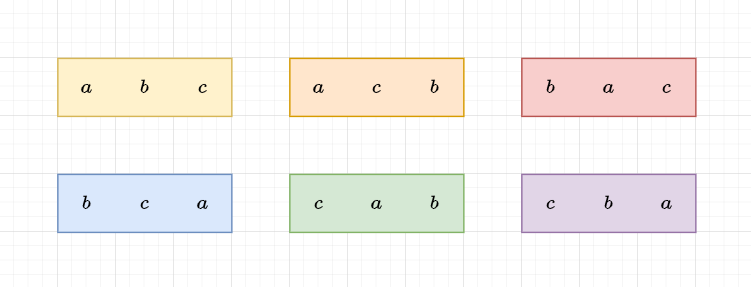
\includegraphics[width=\textwidth]{images/permutation.png}
        \end{center}
    \end{frame}
    
    \begin{frame}{排列 (Permutation)}
        \begin{alertblock}{排列 (Permutation)}
            從 $n$ 個相異元素選出 $r$ 個做排列時,總共有 $P^n_r$ 種不同的排列。 
            \begin{itemize}
                \item $P^n_r = \dfrac{n!}{(n-r)!}$
            \end{itemize}
        \end{alertblock}
    \end{frame}
    
    \begin{frame}{排列 (Permutation)}
        以下從 $\{a,b,c\}$ 中取出 $2$ 個元素做排列時的 $P^3_2 = 6$ 種排列方式
        \begin{center}
            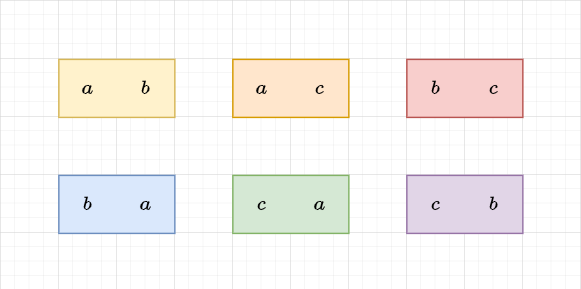
\includegraphics[scale=0.75]{images/nPr.png}
        \end{center}
    \end{frame}
    
    \begin{frame}{排列 (Permutation)}
        \begin{alertblock}{不盡相異物排列}
            有 $n$ 個元素,而每個元素的出現次數共有 $m_i$ 次,則排列的次數一共有
            $$\dfrac{n!}{m_1!m_2!\dots m_k!}$$
        \end{alertblock}
    \end{frame}
    
    \begin{frame}{例題}
        \begin{block}{\href{https://cses.fi/problemset/task/1715}{CSES - Creating Strings II}}
            給你一個字串 $s$,問你有幾個字串可以由 $s$ 經過重組後得到,由於數量可能很大,請輸出答案 $\bmod \ 10^9+7$。
        \end{block} \pause
        基本上就是套剛剛的公式而已,不過由於剛剛有除法以及取模操作,記得要使用模反元素,不能直接用除的!
    \end{frame}
    
    \begin{frame}{組合 (Combination)}
        \begin{alertblock}{組合 (Combination)}
            從 $n$ 個相異元素當中選出 $r$ 個元素的一共有 $C^n_r$ 種
            \begin{itemize}
                \item $C^n_r = \dfrac{n!}{(n-r)!r!}$
                \item $C^n_0 = 1$
                \item $C^n_r = C^n_{n-r}$
                \item $C^n_r$ 又可以被寫成 $\binom{n}{r}$
                \item $C^n_r = C^{n-1}_r + C^{n-1}_{r-1}$ (帕斯卡三角形)
            \end{itemize}
        \end{alertblock}
    \end{frame}
    
    \begin{frame}{組合 (Combination)}
        從 $\{a,b,c\}$ 當中任選 $2$ 個元素的方法,一共有 $C^3_2 = 3$ 種
        \begin{center}
            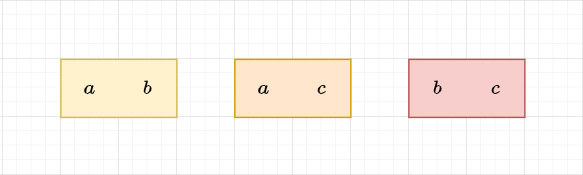
\includegraphics[width=\textwidth]{images/combination.png}
        \end{center}
    \end{frame}
    
    \begin{frame}{組合 (Combination)}
        \begin{alertblock}{重複組合 (Star and Bars)}
            從 $n$ 個元素中取出 $r$ 個,而這 $r$ 個元素可以重複出現,一共有 $H^n_r$ 種選法
            \begin{itemize}
                \item 等同於 $a_1+a_2+\dots+a_n = r$ 的非負整數解數量
                \item 英文稱為 Star and Bars,可以想成是 $r$ 個 $1$ 和 $n-1$ 個 $+$ 在做重複排列
                \item $H^n_r$ 又可以被寫成 $\displaystyle \left(\!\!{\binom {n}{r}}\!\!\right)$
                \item $H^n_r = C^{n+r-1}_{n-1}$ 
            \end{itemize}
        \end{alertblock}
    \end{frame}
    
    \begin{frame}{排容原理 (Inclusion-Exclusion Principle)}
        \begin{alertblock}{排容原理 (Inclusion-Exclusion Principle)}
            若我們有 $n$ 個集合 $A_1,A_2,\dots,A_n$,則
            $$\left|\bigcup^n_{i=1} A_i\right| = \sum_{1 \le i \le n} |A_i| - \sum_{1 \le i < j \le n} |A_i \cap A_j| + \dots + (-1)^{n+1} |A_1 \cap A_2 \cap \dots \cap A_n| $$
            \vspace{5mm}
            \begin{itemize}
                \item $n=2$ 時,有 $|A_1 \cup A_2| = |A_1| + |A_2| - |A_1 \cap A_2|$
                \item $n=3$ 時,有 $|A_1 \cup A_2 \cup A_3| = |A_1| + |A_2| + |A_3| - |A_1 \cap A_2| - |A_2 \cap A_3| - |A_3 \cap A_1| + |A_1 \cap A_2 \cap A_3|$
            \end{itemize}
        \end{alertblock}
    \end{frame}
    
    \begin{frame}{二項式定理 (Binomial Theorem)}
        \begin{alertblock}{二項式定理 (Binomial Theorem)}
            $$(1+x)^n = \binom{n}{0}x^0 + \binom{n}{1}x^1+ \dots + \binom{n}{n}x^n$$
        \end{alertblock}
    \end{frame}
    
    \begin{frame}{例題}
        \begin{block}{\href{https://atcoder.jp/contests/abc178/tasks/abc178_c}{AtCoder Beginner Contest 178C - Ubiquity}}
            請找到有多少個長度為 $N$ 的序列 $A_1,A_2,\dots,A_N$ 滿足
            \begin{itemize}
                \item 對於所有 $i$,$0 \le A_i \le 9$
                \item 至少存在一個 $i$ 使得 $A_i = 0$
                \item 至少存在一個 $i$ 使得 $A_i = 9$
            \end{itemize}
        \end{block} \pause
        \begin{itemize}
            \item 排容原理!
            \item 全部的數量 - (沒有 $0$) - (沒有 $9$) + (沒有 $0$ 也沒有 $9$)
            \item 答案就是 $10^n - 9^n - 9^n + 8^n$
        \end{itemize}
    \end{frame}
    
    \begin{frame}{例題}
        \begin{block}{\href{https://cses.fi/problemset/task/1717}{CSES - Christmas Party}}
            在一個聖誕節派對上,有 $n$ 個人在玩交換禮物,每個人都會送出一個禮物,也會收到一個禮物。請問有幾種送法可以讓這 $n$ 個人都收到不是自己送出去的禮物。
        \end{block}
        \begin{itemize}
            \item<1-> 這個問題其實是經典的「錯排」問題
            \item<2-> 我們可以用排容原理來思考看看
            \item<3-> 答案其實就是 全部 - (至少 $1$ 個人會收到自己的禮物) + (至少 $2$ 個人會收到自己的禮物) - (至少 $3$ 個人會收到自己的禮物) + $\ldots$
            \item<3-> $n! - \sum_{i=1}^n \binom{n}{i} (n-i)!$
        \end{itemize}
    \end{frame}
    
    \begin{frame}{例題}
        \begin{block}{\href{https://codeforces.com/problemset/problem/453/A}{Codeforces 453A - Little Pony and Expected Minimum}}
            你有一個 $m$ 面的均勻骰子,第 $i$ 面上有 $i$ 個點,接著你會骰這個骰子 $n$ 次。而你會將取這 $n$ 次骰出的最大值作為你的分數。請問你得到的分數期望值會是多少? \\
            \vspace{5mm}
            期望值的計算方式為 $\sum X_i \times P_i$
        \end{block} \pause
        \begin{itemize}
            \item<1-> 首先,我們會發現到每個價值的機率其實就是 $(\frac{1}{m})^n$
            \item<2-> 因此,我們只要能夠計算所有情況的價值總和即可
            \item<3-> 那我們要怎麼計算這個答案呢?
            \item<4-> 我們將最大值為 $x$ 的狀態分開思考
        \end{itemize}
    \end{frame}
    
    \begin{frame}{例題}
        \begin{block}{\href{https://codeforces.com/problemset/problem/453/A}{Codeforces 453A - Little Pony and Expected Minimum}}
            你有一個 $m$ 面的均勻骰子,第 $i$ 面上有 $i$ 個點,接著你會骰這個骰子 $n$ 次。而他會將取這 $n$ 次骰出的最大值作為你的分數。請問你得到的分數期望值會是多少? \\
            \vspace{5mm}
            期望值的計算方式為 $\sum X_i \times P_i$
        \end{block} \pause
        \begin{itemize}
            \item<1-> 假設 $n$ 次骰出來的最大值為 $x$,那總共有多少可能呢?
            \item<2-> 排容! 
            \item<3-> 答案其實就是 (其中一次骰出 $x$) - (其中兩次骰出 $x$) + (其中三次骰出 $x$) - \dots
            \item<4-> 不過其實有更簡單的方式! 
            \item<4-> 答案就是 全部 - (沒有骰出 $x$)
            \item<5-> 用一個迴圈跑過每種可能的 $x$ 即可
        \end{itemize}
    \end{frame}
    
    \begin{frame}{例題}
        \begin{block}{\href{https://codeforces.com/problemset/problem/1288/C}{Codeforces 1288C - Two Arrays}}
            現在給你兩個數字 $n,m$,請找出總共有多少對的陣列 $(A,B)$ 滿足
            \begin{itemize}
                \item $A,B$ 的長度皆為 $m$
                \item $1 \le A_i, B_i \le n$
                \item 對於所有 $i$, $A_i \le B_i$
                \item $A$ 陣列是非遞減的 ($A_i \le A_{i+1}$)
                \item $B$ 陣列是非遞增的 ($B_i \ge B_{i+1}$)
            \end{itemize}
        \end{block} \pause
        \begin{itemize}
            \item<1-> 首先,我們觀察到 $A_n \le B_n$,而且 $A$ 是非遞減,$B$ 是非遞增的
            \item<2-> 如果我們知道 $A_i, B_i$ 會有哪些元素,則我們可以知道要怎麼分配這些數字
            \item<3-> $A_1,\dots,A_n,B_n,\dots,B_1$ 會是一個非遞減的陣列
            \item<4-> 我們可以發現 $1 \sim n$ 之間的數字總共出現的頻率會是 $2m$
            \item<5-> $f_1 + f_2 + \dots + f_n = 2m$ 的非負整數解數量!
        \end{itemize}
    \end{frame}
    
    \begin{frame}{例題}
        \begin{block}{\href{Codeforces 893E - Counting Arrays}{https://codeforces.com/problemset/problem/893/E}}
            給你兩個數字 $x,y$,請找出有幾個整數陣列 $F$ 滿足
            \begin{itemize}
                \item $F$ 的長度為 $y$
                \item $\prod^y_{i=1} F_i = x$
            \end{itemize}
        \end{block} \pause
        \begin{itemize}
            \item 將不同的質因數分開思考,假設 $p$ 在 $x$ 的質因數分解中,次方一共是 $cnt_p$ 個
            \item 那我們可以把 $cnt_p$ 分配到 $y$ 個格子裡
            \item 直接使用重複組合的公式即可!
        \end{itemize}
    \end{frame}
    
    \begin{frame}{例題}
        \begin{block}{2020 北市賽 pC - 婚禮的裝飾}
            有 $n$ 個格子,每個格子可以擺上 $6$ 種棋子中的其中一種 (國王、皇后、主教、騎士、士兵、城堡),請問有幾種擺法可以使國王和皇后的出現次數皆為偶數?
            \begin{itemize}
                \item $1 \le n \le 10^9$
            \end{itemize}
        \end{block}
        \begin{itemize}
            \item 跟矩陣快速冪同一題,但這次我們要用數學!
        \end{itemize}
    \end{frame}
    
    \begin{frame}{例題}
        \begin{block}{2020 北市賽 pC - 婚禮的裝飾}
            有 $n$ 個格子,每個格子可以擺上 $6$ 種棋子中的其中一種 (國王、皇后、主教、騎士、士兵、城堡),請問有幾種擺法可以使國王和皇后的出現次數皆為偶數?
            \begin{itemize}
                \item $1 \le n \le 10^9$
            \end{itemize}
        \end{block}
        \begin{itemize}
            \item<1-> 這題 $n$ 很大,不過我們先想想看,如果 $n \le 10^3$ 要怎麼處理呢?
            \item<2-> 枚舉國王與皇后的出現次數!
            \item<3-> 答案會是 $\displaystyle \sum_{0 \le i \le n, i \text{ odd}} \binom{n}{i}\sum_{0 \le j \le n-i, j \text{ odd}} \binom{n-i}{j} 4^{n-i-j}$
        \end{itemize}
    \end{frame}
    
    \begin{frame}{例題}
        \begin{block}{2020 北市賽 pC - 婚禮的裝飾}
            有 $n$ 個格子,每個格子可以擺上 $6$ 種棋子中的其中一種 (國王、皇后、主教、騎士、士兵、城堡),請問有幾種擺法可以使國王和皇后的出現次數皆為偶數?
            \begin{itemize}
                \item $1 \le n \le 10^9$
            \end{itemize}
        \end{block}
        \begin{itemize}
            \item<1-> 如果 $n \le 10^6$ 呢?
            \item<2-> 我們把裡面的東西抓出來看看
            \item<2-> $\displaystyle \sum_{0 \le j \le n-i, j \text{ odd}} \binom{n-i}{j} 4^{n-i-j}$
            \item<3-> 欸? 是不是很像二項式定理呢? ($(1+x)^n = \sum_{i=0}^n \binom{n}{i} x^i$)
            \item<4-> 其實上式可以被化簡為 $((1+4)^{n-i} + (1-4)^{n-i})/2$ ($n$ 是偶數) 
            \item<4-> 或 $((1+4)^{n-i} - (1-4)^{n-i})/2$ ($n$ 是奇數)
        \end{itemize}
    \end{frame}
    
    \begin{frame}{例題}
        \begin{block}{2020 北市賽 pC - 婚禮的裝飾}
            有 $n$ 個格子,每個格子可以擺上 $6$ 種棋子中的其中一種 (國王、皇后、主教、騎士、士兵、城堡),請問有幾種擺法可以使國王和皇后的出現次數皆為偶數?
            \begin{itemize}
                \item $1 \le n \le 10^9$
            \end{itemize}
        \end{block}
        \begin{itemize}
            \item 因此在 $n \le 10^6$ 時
            \item 直接套 $\displaystyle \sum_{0 \le i \le n, i \text{ odd}} \binom{n}{i} ((1+4)^{n-i} + (1-4)^{n-i})/2$ ($n$ 是偶數) 
            \item 或 $\displaystyle \sum_{0 \le i \le n, i \text{ odd}} \binom{n}{i} ((1+4)^{n-i} - (1-4)^{n-i})/2$ ($n$ 是奇數) 即可
        \end{itemize}
    \end{frame}
    
    \begin{frame}{例題}
        \begin{block}{2020 北市賽 pC - 婚禮的裝飾}
            有 $n$ 個格子,每個格子可以擺上 $6$ 種棋子中的其中一種 (國王、皇后、主教、騎士、士兵、城堡),請問有幾種擺法可以使國王和皇后的出現次數皆為偶數?
            \begin{itemize}
                \item $1 \le n \le 10^9$
            \end{itemize}
        \end{block}
        \begin{itemize}
            \item<1-> 那在 $n \le 10^9$ 的時候怎麼辦呢?
            \item<2-> 我們將剛剛化簡的式子再進一步地化簡 (在此省略 $n$ 是奇數的 case)
            \item<3-> $\displaystyle \frac{1}{2}(\sum_{0 \le i \le n, i \text{ odd}} \binom{n}{i} (1+4)^{n-i} + \sum_{0 \le i \le n, i \text{ odd}} \binom{n}{i} (1-4)^{n-i})$
            \item<4-> 再套一次二項式定理!
        \end{itemize}
    \end{frame}
    
    \begin{frame}{例題}
        \begin{block}{2020 北市賽 pC - 婚禮的裝飾}
            有 $n$ 個格子,每個格子可以擺上 $6$ 種棋子中的其中一種 (國王、皇后、主教、騎士、士兵、城堡),請問有幾種擺法可以使國王和皇后的出現次數皆為偶數?
            \begin{itemize}
                \item $1 \le n \le 10^9$
            \end{itemize}
        \end{block}
        $$\displaystyle \frac{1}{2}(\sum_{0 \le i \le n, i \text{ odd}} \binom{n}{i} (1+4)^{n-i} + \sum_{0 \le i \le n, i \text{ odd}} \binom{n}{i} (1-4)^{n-i})$$
        $$\displaystyle \frac{1}{2} (((1+5)^n - (1-5)^n)/2 + ((1-3)^n - (1+3)^n)/2)$$
        $$\displaystyle \frac{1}{4} ((6^n - (-4)^n) + ((-2)^n - 4^n))$$
    \end{frame}
    
    
    \begin{frame}{例題}
        \begin{block}{2020 北市賽 pC - 婚禮的裝飾}
            有 $n$ 個格子,每個格子可以擺上 $6$ 種棋子中的其中一種 (國王、皇后、主教、騎士、士兵、城堡),請問有幾種擺法可以使國王和皇后的出現次數皆為偶數?
            \begin{itemize}
                \item $1 \le n \le 10^9$
            \end{itemize}
        \end{block}
        \begin{itemize}
            \item<1-> 因此最後的一般式就是 $\displaystyle \frac{1}{4} (6^n - (-4)^n + (-2)^n - 4^n)$ ($n$ 是偶數)
            \item<1-> 或 $\displaystyle \frac{1}{4} (6^n + (-4)^n - (-2)^n - 4^n)$ ($n$ 是奇數)
            \item<1-> 只要使用快速冪就能在 $O(\log n)$ 計算完成了!
        \end{itemize}
    \end{frame}
    
\end{document}